\documentclass{report}
\usepackage{graphicx}
\usepackage{listings}
\begin{document}
	\textbf{Partner Info: Shaan Mehta(20510804)}\\\\
	\begin{enumerate}
		\item{The order doesnt matter because in non-blocking assignment the simulator will wait until all the right-hand side variables are stable before assigning the value to the left-hand side variables. So as long as all 3 statements are contained in the always block, our output will be the same regardless of the ordering.}
	
		\item{
			The first the input signal "in" will pass through an adder and into data input of register X. Adder 1 will increment the input by 1. Output of adder 1 will go to adder 2 and data input of register Y. Adder 2 will also increment its input by one. Output of adder 3 will be connected to data input of register Z.\\
			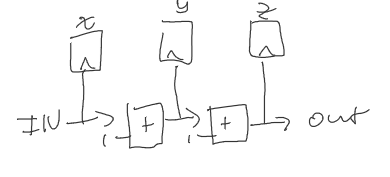
\includegraphics[scale=0.5]{hw_diag}\\\\
		}
		
		\item{
			We add the reset signal to the sensitivity list of the always block in and\_reg. This means that the block will be triggered outside of the rising edge of the clock if the reset signal is flipped if the reset signal is high then the register will be reset.\\
			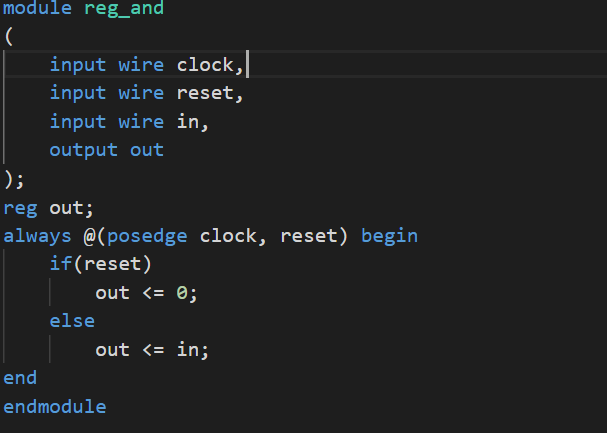
\includegraphics[scale=0.5]{async_reset}\\\\
		}
		\pagebreak\\
		\item{
			\begin{lstlisting}[language=verilog]
				module dut;
				reg x, y, reset;
				reg clock = 1;
				wire z, x_reg, y_reg, out;
				
				initial begin
				$dumpfile("reg-and.vcd");
				$dumpvars(0, gate);
				$dumpvars(0, reg_gate);
				
				#0 reset = 1;
				#20 x = 0; y = 0;
				reset <= 0; $display("Reset complete");
				#10 x = 1; y = 1; $display("set 1 1");
				#10 x = 1; y = 0;
				#10 x = 1; y = 1;
				#10 x = 0; y = 1;
				#20 $finish;
				end
				
				and_assign gate (.x(x_reg), .y(y_reg), .z(z));
				reg_and reg_gate (.clock(clock), .reset(reset), .in(z), .out(out));
				reg_and reg_gate_in_x (.clock(clock), .reset(reset), .in(x), .out(x_reg));
				reg_and reg_gate_in_y (.clock(clock), .reset(reset), .in(y), .out(y_reg));
				
				always begin
				#5 clock = ~clock;
				end
				
				always @(posedge clock) begin
				$display("time=%t, reset=%b, x=%b, x_reg=%b, y=%b, y_reg=%b, z=%b, out=%b", $time,reset,x, x_reg, y, y_reg, z, out);
				end
				endmodule 
			\end{lstlisting}\\
			And the output:\\
			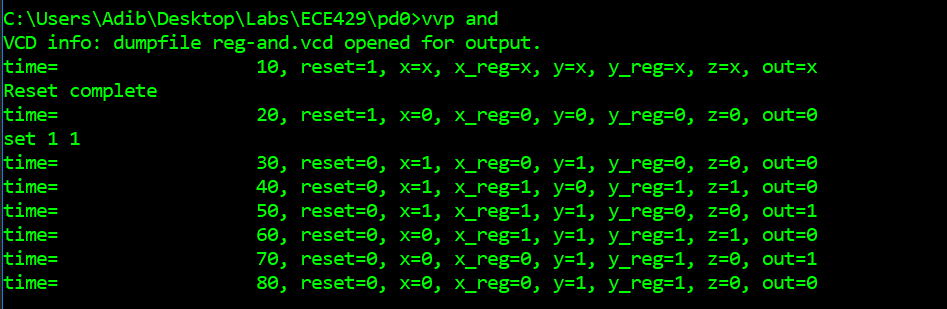
\includegraphics[scale=0.5]{reg_insert_output}\\\\
			The simulated output shows the expected behaviour. For a given x,y pair input to the and gate the correct output z is delayed by one cycle. This is because the input pair is initially registered and then in the next cycle the registered values are passed to the and gate.
		}
	\end{enumerate}
\end{document}